
\documentclass[12pt]{article}
\usepackage[numbers,sort]{natbib}
\usepackage{amsfonts,amsmath}
\usepackage{graphicx}
\usepackage{libertine}
\usepackage{fullpage}
\usepackage{hyperref}
\hypersetup{colorlinks=true,linkcolor=blue,urlcolor=blue,citecolor=blue,anchorcolor=blue}
\urlstyle{same}

\begin{document}

\begin{center}
    {\Large\bfseries
    LLM-Guided Heuristic Discovery for Online Bin Packing:
    Independent Sampling versus Evolutionary Feedback
    \par}

    \vspace{0.2cm}
    {\normalsize \today}

    \vspace{0.2cm}

    \begin{tabular}{cccc}
        Gabrielle Lau Qian Tong & Nicole Neo Xin Hui &
        Stuti Kansal & Valerie Lim \\
        A0283288N & A0282252J &
        A0281988E & A0282819R
    \end{tabular}

    \vspace{0.2cm}

    \textbf{GitHub Repository:}
    \url{https://github.com/neo-nicole/dsa4212-group11}
\end{center}

\vspace{0.1cm}

\section{Introduction and Related Work}
Large language models (LLMs) have propelled the automated discovery of optimisation heuristics through program search. In LLM-guided search, an LLM generates candidate programs under specified constraints, an evaluator scores them on problem instances, and the best-scoring programs are retained. For independent sampling, the LLM is queried repeatedly with the same prompt. Evolutionary approaches additionally feed promising candidates back into subsequent prompts so that the LLM is able to iteratively refine them. This is demonstrated in FunSearch, which uses this approach to evolve priority functions for online bin packing, achieving performance improvements over established baselines such as First Fit and Best Fit \citep{romera2023}.

Despite promising results, LLM-guided evolutionary search may incur significant discovery costs from repeated LLM inferences to generate candidate programs iteratively. Furthermore, by incorporating previously discovered promising candidates in the generation prompts, each call consumes more tokens compared to independent sampling. As a result, comparing independent sampling and evolutionary feedback using a fixed number of LLM calls may not accurately reflect computational expenditure due to differences in token consumption, possibly inflating the benefits of evolutionary feedback. FrugalEvo emphasises the importance of evaluating evolutionary search by solution quality relative to cost instead of by a fixed iteration number \citep{chen2026}. This motivates the investigation of whether evolutionary feedback provides meaningful gains over independent sampling under controlled token budget constraints.

Another consideration when evaluating discovered heuristics is its generalisability. Although FunSearch demonstrated that its evolved heuristics transferred across problem sizes, evolution and evaluation was conducted within the same distribution family, and generalisation on unseen distributions remains unestablished. In particular, as evolutionary feedback selects candidates by training performance and incorporates them into subsequent prompts, the heuristics discovered may exploit characteristics specific to the training distribution \citep{huang2025}. Although this can improve in-distribution performance, LLM-evolved heuristics have been found to generalise poorly when evaluated across a broad range of benchmarks \citep{sim2025}. This motivates evaluating transfer to unseen instance sizes and distributions.

In this study, we investigate these gaps using one-dimensional online bin packing, comparing independent sampling (Method A) and evolutionary feedback (Method B). Both methods start from the same Best Fit program, and are compared against First Fit, Best Fit and ab-First Fit as baselines. Specifically, we address the following research questions:
\begin{enumerate}\item Under a fixed LLM token budget, does evolutionary feedback discover better online bin-packing heuristics than independent sampling?
\item Does evolutionary feedback affect how well discovered heuristics generalise to unseen item-size distributions, instance sizes and item orderings?\end{enumerate}



\section{Problem Formulation}

In one-dimensional online bin packing, each item is only
seen as it arrives. The item is then assigned to an
existing bin, or a new bin is opened, depending on the
item's size and remaining bin capacity. The objective
is to minimise the total number of bins.

Thus, we used LLM-guided evolution to evolve a
bin-selection rule, where the heuristic is a priority
function \textttt{priority\_fn(item\_size,
open\_bin\_remaining\_capacities, capacity)}.
Here, \textttt{item\_size} is the size of the current
item, \textttt{open\_bin\_remaining\_capacities}
represents the available space in each existing bin
that can fit the incoming item, and \textttt{capacity}
is the fixed maximum bin capacity of 100.
The function returns a score for each bin and one
score for opening a new bin, and the simulator
places the item in the highest-scoring bin.

Each candidate program was then scored using
percentage excess over the lower bound, defined as
$\text{score} = 100 \times (B-L)/L$,
where $B$ is the number of bins used and
$L = \left\lceil \sum_i x_i / C \right\rceil$
is the theoretical lower bound, with $x_i$
representing item sizes and $C=100$ is the bin capacity.
Scores are evaluated within each family and across
families, where a lower score is better.


\section{Methodology}

\begin{figure}[htbp]
    \centering
    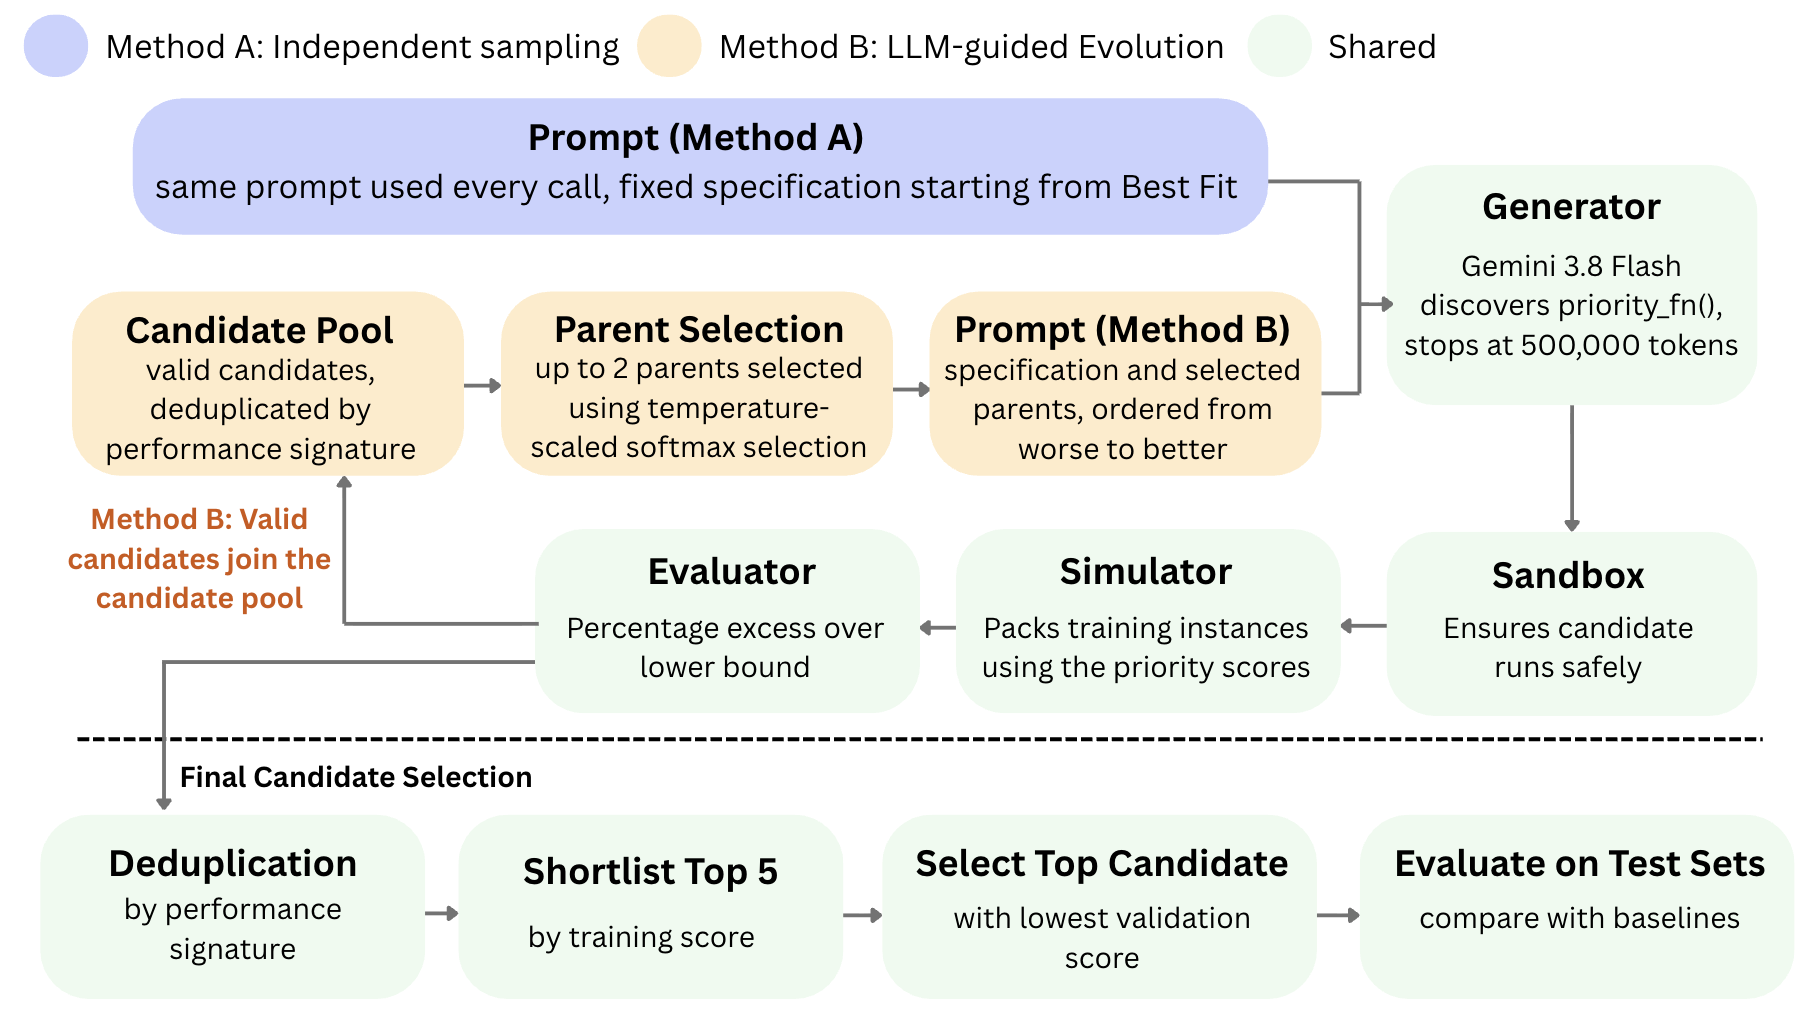
\includegraphics[width=0.75\linewidth]{images/Figure 1.png}
    \caption{Pipeline overview of Methods A and B}
    \label{fig:pipeline}
\end{figure}


Each method and repetition received an independent token ceiling of 500,000 tokens. The search stopped when the next request could not fit within the remaining ceiling.

\subsection{Method A: Independent Sampling}
Method A uses independent sampling of the LLM-generated candidate programs. For each LLM call, the LLM receives the common specification prompt and Best Fit as the starting program from method\_a.py, and then generates a new standalone priority\_fn(). The candidate is extracted and checked for valid syntax/signature, and runs in the sandbox on the training instances. After which, its bin-packing score, validity, token usage, and cost are logged. The valid candidates are then deduplicated, before the top five by training score are shortlisted, and the one with the best validation score is selected as the overall best program.

\subsection{Method B: LLM-guided evolution}
In Method B, each generation call likewise starts with the Best Fit function as the initial candidate. In addition, a population of valid candidate priority\_fn()s was maintained, with behavioural duplicates removed using each candidate's per-instance score signature. If the performance signature was the same, then the shortest candidate was kept. 2 parents were then sampled with replacement using their training scores, using a temperature-scaled softmax selection for minimising the scores, where selection temperature was (T=1.0).

\begin{equation}\label{eq:weight} w_i = \exp\!\left(-\frac{s_i-s_{\min}}{T}\right)\end{equation}

where $w_i$ is candidate $i$'s selection weight, $s_i$ is candidate $i$'s training score, $s_{min}$ is the lowest current training score, and $T$ is the selection temperature.

The selection probability for candidate $i$ is then obtained by normalising its weight across all candidates. Hence, candidates that resulted in lower percentage excess over the theoretical lower bound received larger weights and therefore had higher selection probabilities, but the temperature still allows exploration.

After this, the selected parent functions were shown to the LLM, ordered from worse to better. Using these parents, a new standalone child priority\_fn() was generated, then sandboxed, and evaluated on the training set. Valid children are then added to the population and may become future parents. This continues until the token budget is exhausted.

Like Method A, after all the candidates have been generated, candidates were deduplicated again, the top five by training score were shortlisted, and the candidate with the best validation score was selected.
\section{Experimental Setup}
\subsection{Data Splits}

Table~\ref{tab:splits} summarises the training, validation, and test splits. All instances use bin capacity of 100 and integer item sizes. Training instances were used to generate and score candidate priority\_fn()s, while validation instances were used solely for final candidate selection to prevent selecting a candidate based only on training performance. The in-distribution (ID) test set contains the same distributions as the train set but with different item sequences, while the out-of-distribution (OOD) test set evaluates transfer across unseen sequence lengths, orderings and distributions. To prevent instance-level data leakage, different seeds were used to create different random instances while keeping the distributions consistent, ensuring that training and validation instances did not overlap. The sorted ascending and descending OOD families used the same underlying random items, so any performance difference could be attributed to item ordering rather than different item values.



\begin{table}[htbp]\centering\small
\caption{Data splits and corresponding instance distributions}\label{tab:splits}
\begin{tabular}{p{0.19\linewidth}p{0.52\linewidth}rr}\hline
Split & Family distribution & Per family & Total \\\hline
Train & Uniform item sizes 1--100; 200 or 500 items & 30 & 60 \\
Validation & Same uniform families, different seeds & 15 & 30 \\
ID test & Same uniform families, different seeds & 20 & 40 \\
OOD test & Weibull; mostly large; near-identical; uniform 100 or 1000 items; largest-first and smallest-first orderings & 20 & 140 \\\hline
\end{tabular}\end{table}

\subsection{Sandbox Evaluation}
The sandbox provided process-isolation for evaluating for LLM-generated heuristics. It validated each candidate’s syntax and required \textttt{priority\_fn} interface, restricted available built-ins and imports, and enforced execution timeouts. This prevented malformed, failing, or excessively slow candidates from disrupting the experiments and ensured that candidates were evaluated consistently using the same simulator and scoring metric. The sandbox was used during training search, validation-based candidate selection, and final evaluation on both ID and OOD test sets. Note that it was not intended to provide security-grade isolation for arbitrary untrusted code.

\subsection{LLM Configurations and Runtime Settings}

\begin{table}[htbp]\centering\caption{LLM configuration and runtime settings}\label{tab:settings}
\begin{tabular}{ll}\hline Setting & Value \\\hline
Model & \textttt{google/gemini-3.8-flash} \\
LLM sampling temperature & 1.0 \\
Reasoning effort & Low \\
Maximum output tokens per call & 2000 \\
Token budget & 500,000 per method per run \\
Search timeout & 10 s \\\hline\end{tabular}\end{table}
Identical configurations are used for both Method A and Method B experiments (Table~\ref{tab:settings}). The LLM sampling temperature of 1.0 encourages exploration of more diverse candidate programs, while low reasoning effort enables fast inference and reduces inference costs. Each run is limited to 500,000 tokens, including prompt and output tokens, instead of a fixed number of calls. Candidate evaluation on the training set is capped at 10s during search, rejecting excessively slow programs.

\subsection{Baselines}
Before we implemented the LLM evolution loop, we first implemented common bin-packing heuristics, First Fit and Best Fit, as well as tuned ab-First Fit (ABFF) \citep{herrmann2026}. These baselines serve as a reference point for comparison on solution quality, generalisation across distributions, execution time and whether the LLM-generated heuristics for either methods improve over established baselines. Best Fit in particular was used as the starting candidate program for both Method A and B, as previously mentioned.

\subsubsection{Tuning of ab-First Fit}

ABFF combines Best Fit and First Fit using two thresholds,
$a$ and $b$. For each feasible bin, the gap was calculated
as $\text{gap} = \text{remaining capacity} - \text{item size}$.
For each value of the gap:

\begin{itemize}
    \item If $\text{gap} \leq a$, a Best Fit-style priority was used.
    \item If $\text{gap} \geq b$, a First Fit-style priority was used.
    \item If $a < \text{gap} < b$, the bin was avoided.
    \item If no suitable bin was selected, a new bin was opened.
\end{itemize}

A grid search was performed over all integer pairs
$(a,b)$ satisfying $0 \leq a < b$, $a \leq 30$,
and $b \leq 45$. For every $(a,b)$ pair, ABFF was
evaluated on all training instances and scored using
the mean percentage excess over the lower bound.
The scores were averaged across distribution families,
and the pair with the lowest mean training score was
selected. The final selected parameters were
$(a,b) = (11,35)$.


\subsection{Pilot Runs}
We ran 2 pilot runs to determine practicalities such as to gauge cost, assess any implementation gaps, and parameter selection.

\subsubsection{Pilot 1}
Pilot 1 ran 50 calls per method, with both methods starting from scratch, instead of being given Best Fit as a starting candidate program. Method B also followed a linear selection of the parent candidate program, where the latest child candidate automatically became the next parent candidate. Neither methods improved upon Best Fit, leading us to realise two limitations: the lack of a baseline heuristic for the LLM to evolve on, unlike FunSearch, potentially led to the rediscovery of Best Fit, instead of discovering improved heuristics; in Method B, exploration was limited as we constantly evolved on the latest candidate, instead of maintaining a candidate pool and sampling parent candidates to generate future child candidates.

To improve selection, we implemented a soft-max selection rule to select the parent candidates, and test different selection temperatures for Method B in Pilot 2, to strike a better balance between exploitation and exploration. We also moved from only considering the aggregate score of each candidate (the total score averaged across all instances), to considering per-instance performance signatures when choosing and deduplicating candidates.

\subsubsection{Pilot 2}
Pilot 2 ran 300 calls per method. Adopting FunSearch's design, Best Fit was now the starting candidate program, with performance signatures of candidates taken into account to deduplicate candidate programs. Parent selection temperatures of $T \in \{0.1, 0.5, 1.0\}$ were compared and a candidate pool was maintained for Method B (Figure~\ref{fig:pilot}).

\begin{figure}[htbp]
    \centering
    \begin{minipage}{0.48\textwidth}
        \centering
        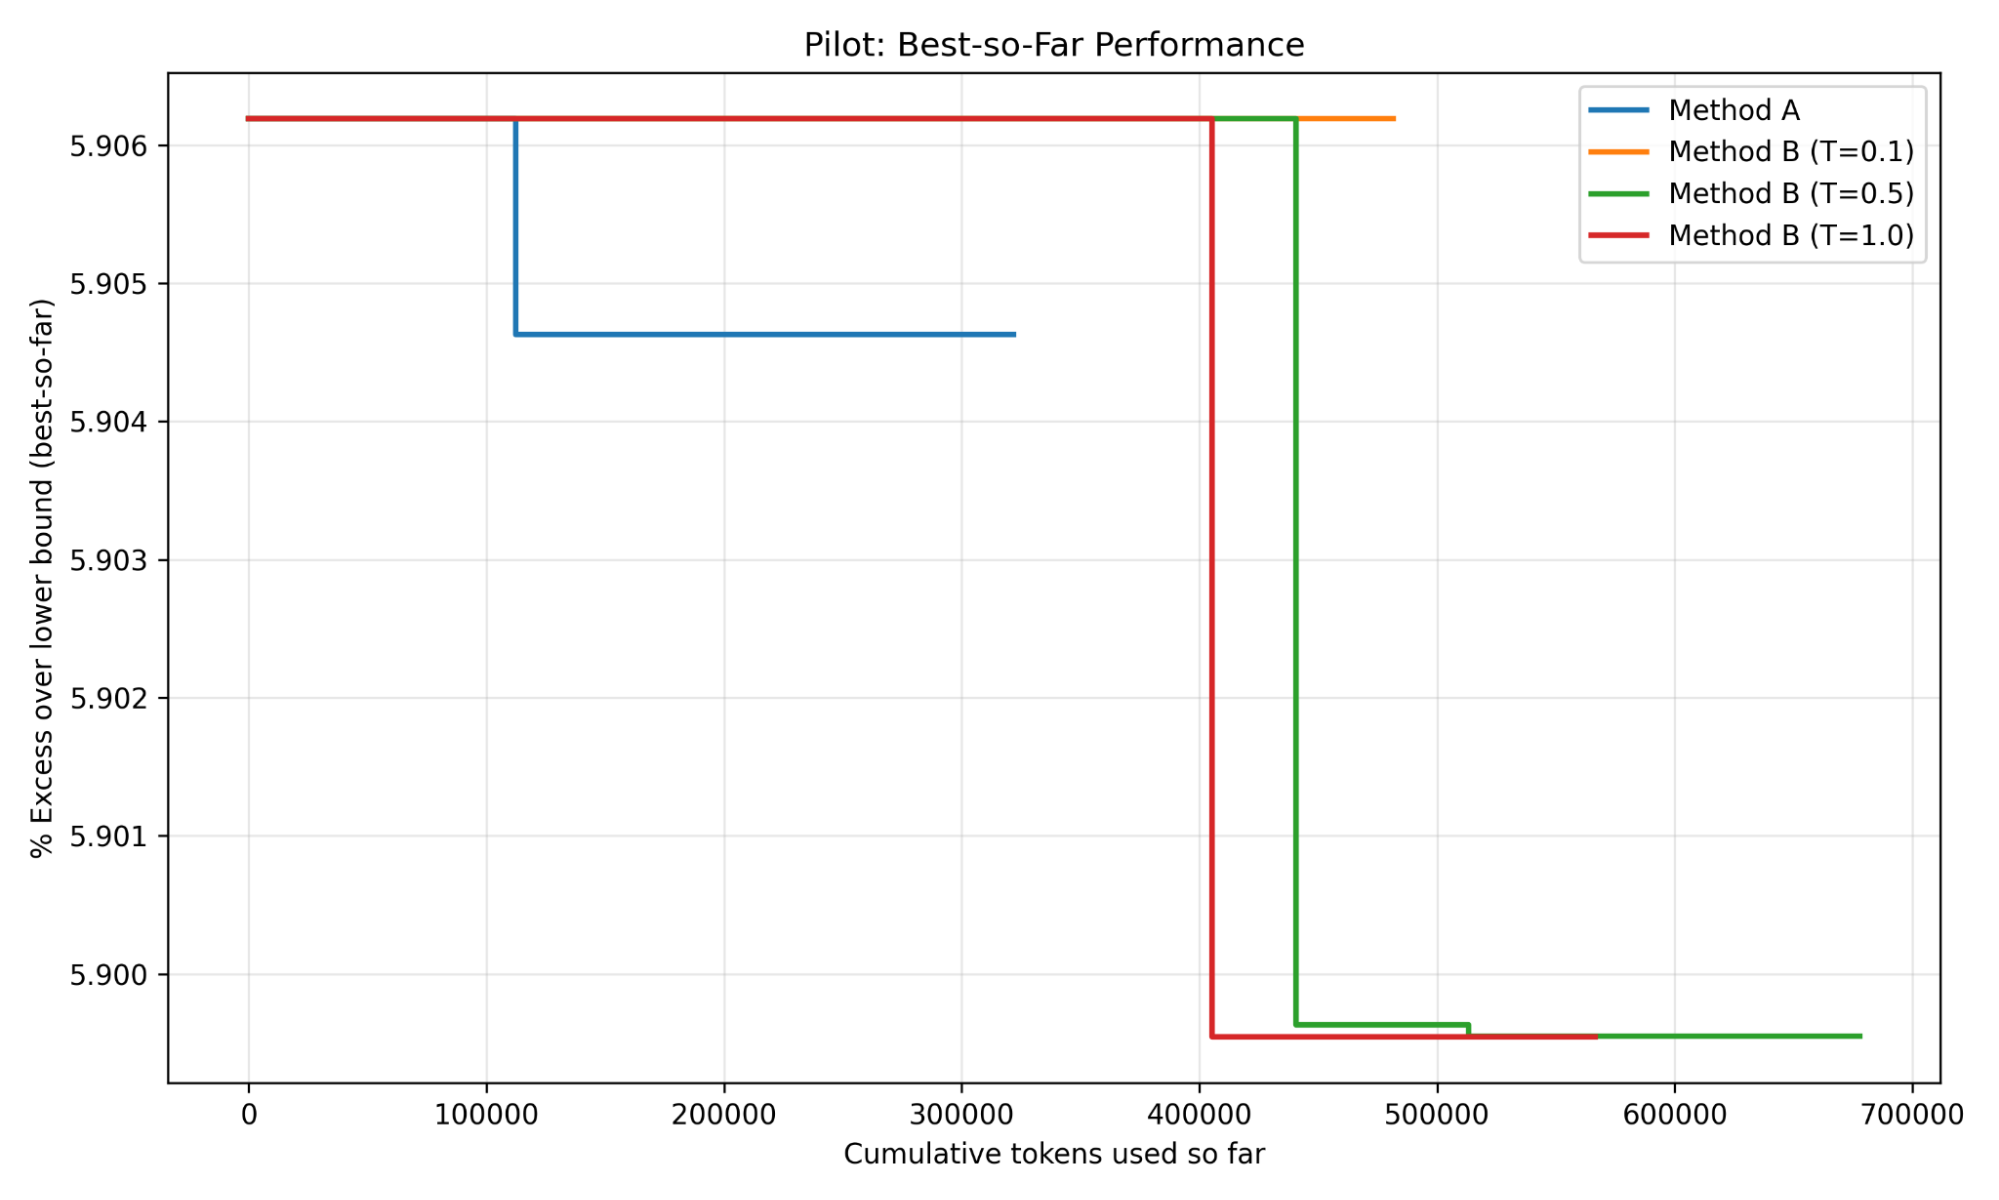
\includegraphics[width=\linewidth]{images/Figure 2(a).png}
        \small (a) Best-so-far score
    \end{minipage}
    \hfill
    \begin{minipage}{0.48\textwidth}
        \centering
        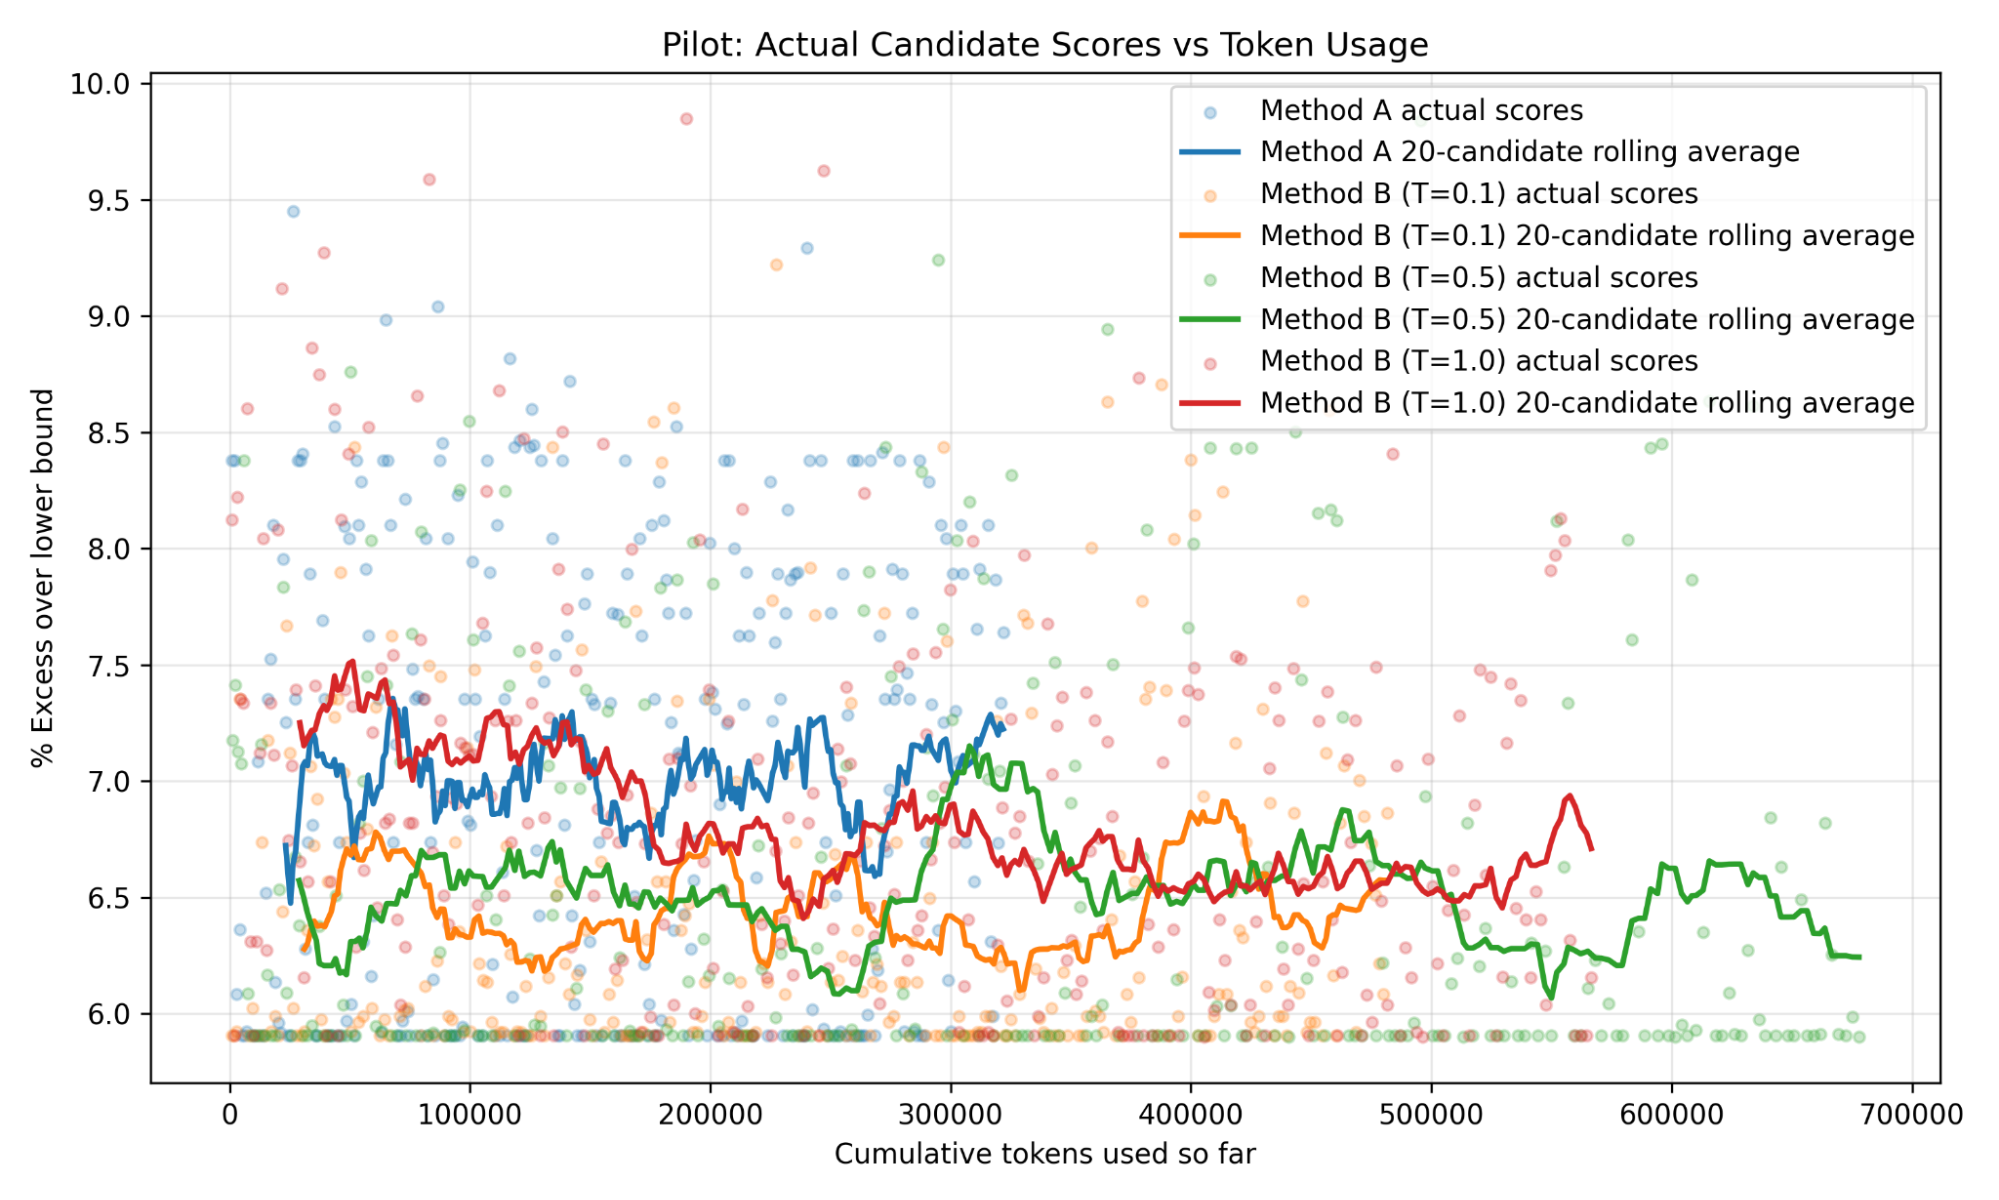
\includegraphics[width=\linewidth]{images/Figure 2(b).png}
        \small (b) Mean excess score
    \end{minipage}
    \caption{Pilot 2: (a) best-so-far score and (b) mean excess score against cumulative tokens used.}
    \label{fig:pilot}
\end{figure}

Best-so-far performance was plotted against cumulative tokens used to inform budget selected (Figure~\ref{fig:pilot}). The best-so-far score rarely changed, with Method A improving once at about 110,000 tokens, while Method B saw improvements at 400,000-500,000 tokens. Hence, we set our final run token budget at 500,000 tokens. At (T=1.0), Method B used  76\% more tokens per call than Method A (1888 versus 1073) as each prompt included parent programs. Thus, we budgeted by token count instead of the number of calls for our final runs. We selected (T=1.0) based on the pilot validation analysis and its exploration-oriented parent selection. In particular, the validation analysis found that (T=1.0) beat Best Fit, exposed substantially more distinct parents than (T=0.1) (151 versus 50), and produced only one invalid candidate. The pilot also estimated roughly \$1.40 for each run pair, with LLM spending being the binding constraint while candidate evaluation ran locally with negligible cost. Furthermore, as Best Fit evaluated on the train split well within 10s, we kept the 10s search timeout.

\subsection{Main Experiment}
For our final runs, we performed 2 repetitions of each method, with seed=1 and seed=2, where candidate programs were generated and scored on the training set, while candidate selection was done on the validation set. We summarise each run by its LLM calls, valid candidates, tokens, cost, and best and mean train score (Table~\ref{tab:runs}). Each run's selected heuristic is then evaluated on the ID test set, OOD test set, and compared to our baselines -- First Fit, Best Fit and Tuned ABFF. Heuristics are compared using the total bins used relative to Best Fit on the same instance family (Table~\ref{tab:tests}). As both methods start from Best Fit, we can observe how much each search improves on its starting program.

\section{Results}
Table~\ref{tab:runs} summarises the candidate generation performance across the four experimental runs. Method B achieved a lower mean training score than Method A across both repetitions. For seed 1, Method B achieved a mean score of 6.858, compared to 7.054 for Method A. Similarly, for seed 2, Method B achieved a mean score of 6.822, compared to 6.943 for Method A.
However, Method A achieved marginally better best training scores in both repetitions, with a score of 5.905 compared to 5.906 for Method B. In terms of candidate generation, Method A also produced more valid candidates (471 and 481) than Method B (267 and 230), despite both methods consuming approximately the same token budget.

\begin{table}[htbp]\centering\scriptsize\caption{Score and cost per experimental run}\label{tab:runs}
\resizebox{\textwidth}{!}{\begin{tabular}{lrrrrrrl}\hline
Run & LLM calls & Valid candidates & Tokens & Cost (USD) & Best train score & Mean train score & Selected heuristic \\\hline
A, seed 1 & 479 & 471 & 494167 & 0.814 & 5.905 & 7.054 & Best Fit \\
A, seed 2 & 484 & 481 & 494830 & 0.806 & 5.905 & 6.943 & Best Fit \\
B, seed 1 & 267 & 267 & 492238 & 0.721 & 5.906 & 6.858 & Best Fit \\
B, seed 2 & 261 & 230 & 492034 & 0.723 & 5.906 & 6.822 & Best Fit \\\hline
\end{tabular}}\end{table}

\begin{table}[htbp]\centering\scriptsize\caption{Test results relative to Best Fit. Comparison columns report differences in total bins used.}\label{tab:tests}
\resizebox{\textwidth}{!}{\begin{tabular}{llrrrr}\hline
Test & Family & BF excess (\%) & FF vs BF & ABFF vs BF & A/B vs BF \\\hline
ID & Uniform, 200 items & 8.015 & 24 & -12 & 0 \\
ID & Uniform, 500 items & 4.849 & 66 & 1 & 0 \\
OOD & Weibull, 200 items & 5.802 & 7 & 0 & 0 \\
OOD & Mostly large [50,100], 200 items & 31.757 & 0 & 0 & 0 \\
OOD & Near identical [40,45], 200 items & 16.758 & 0 & 1395 & 0 \\
OOD & Uniform, 100 items & 8.970 & 12 & -2 & 0 \\
OOD & Uniform, 1000 items & 4.132 & 132 & 4 & 0 \\
OOD & Sorted largest-first, 200 items & 2.846 & 0 & 37 & 0 \\
OOD & Sorted smallest-first, 200 items & 27.671 & 0 & -109 & 0 \\\hline
\end{tabular}}\end{table}





Table~\ref{tab:tests} presents the test performance of the selected heuristics relative to Best Fit across the ID and OOD test families. Across all 4 runs, Best Fit was selected as the final heuristic after validation-based selection. Consequently, both methods achieved identical test performance to Best Fit across all evaluation families, meaning neither method produced a final heuristic that improved upon its starting program, despite using approximately 500,000 tokens per run.


In Figure~\ref{fig:main}(a), Method A achieved marginal improvements in its best-so-far training score during the search, whereas Method B remained relatively flat across both repetitions. In particular, Method A achieved a best score of around 5.9046, compared to approximately 5.9062 for Method B. Neither method demonstrated substantial improvements as cumulative token consumption increased. Both methods also plateaued relatively early, suggesting that additional token expenditure did not translate into meaningful improvements in the best candidate discovered.
Figure~\ref{fig:main}(b) shows that Method B achieved a lower mean candidate score than Method A, while both methods had similar median scores. Method B also exhibited a narrower interquartile range, indicating less variation in its generated candidate scores.


\begin{figure}[htbp]
    \centering
    \begin{minipage}{0.48\textwidth}
        \centering
        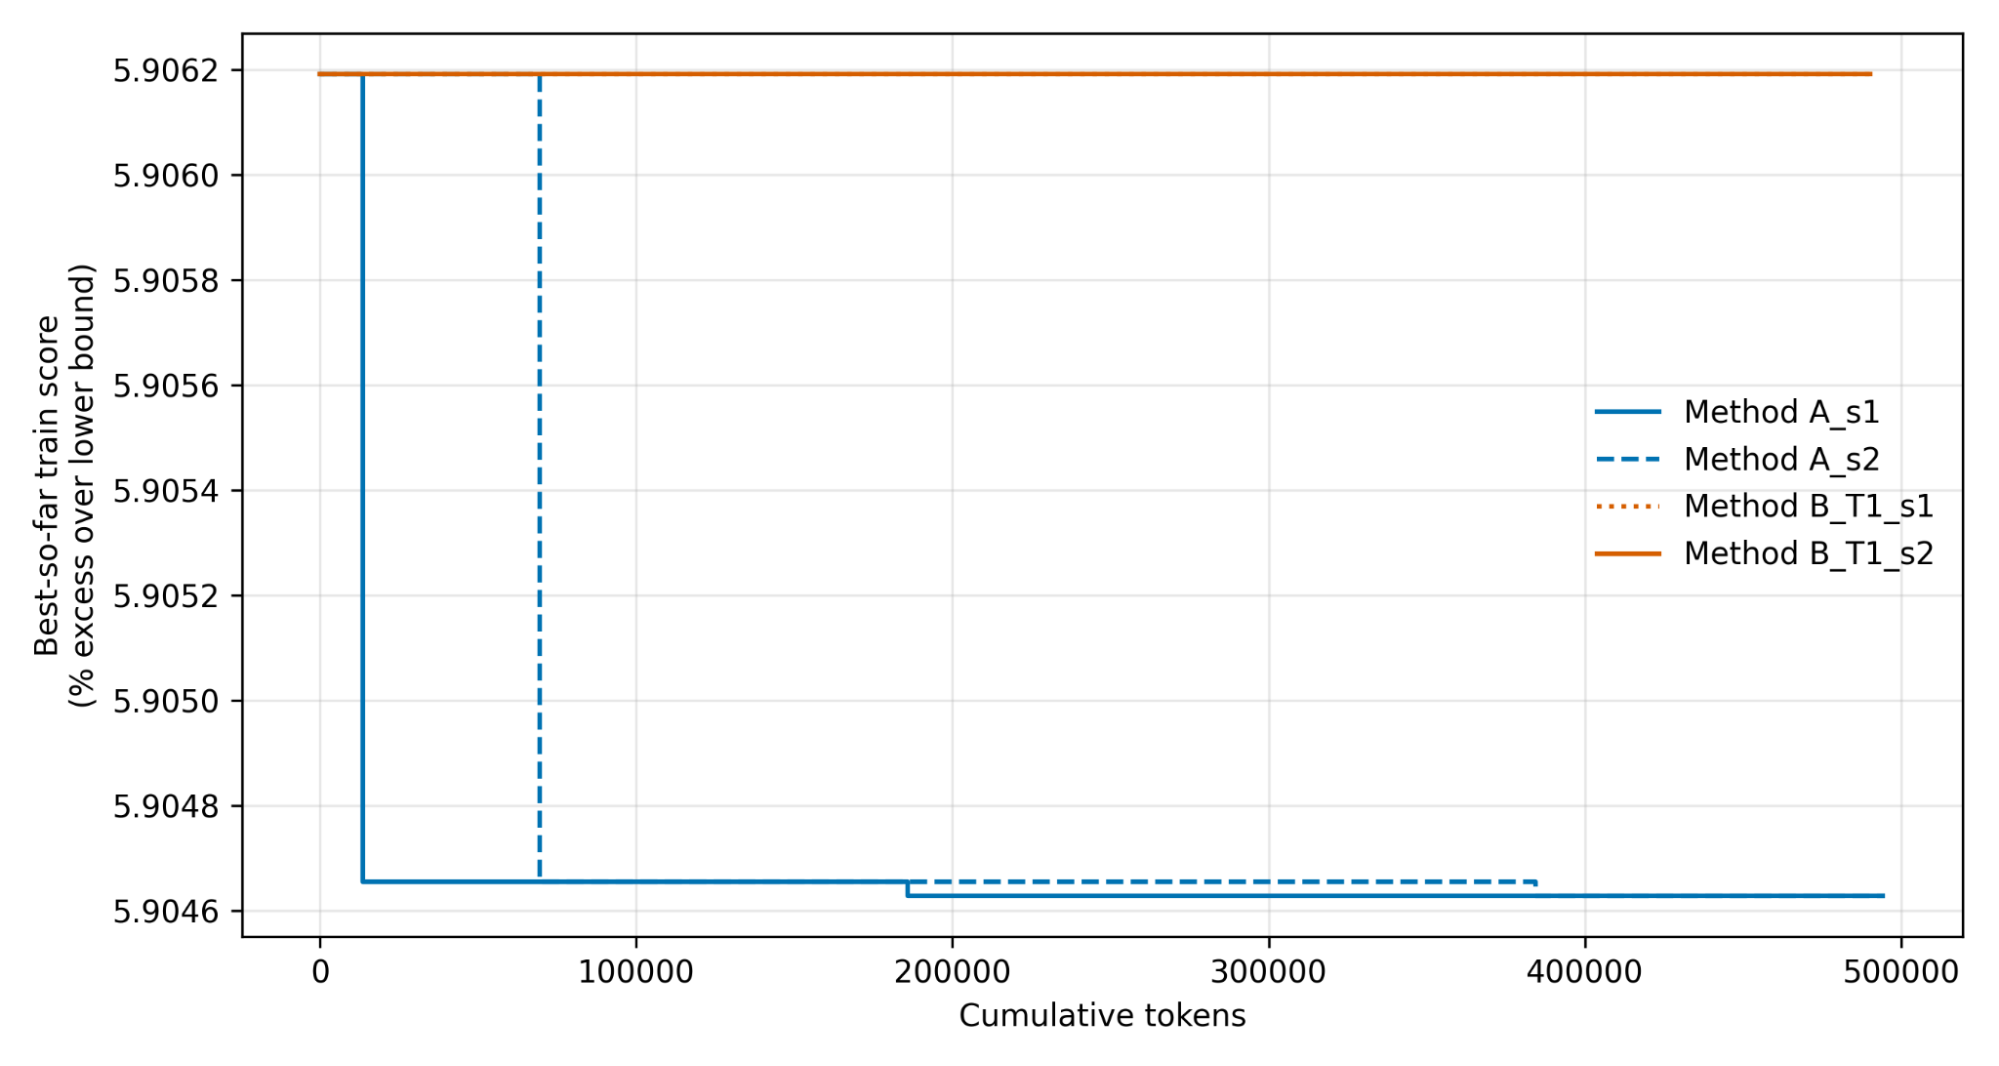
\includegraphics[width=\linewidth]{images/Figure 3(a).png}
        \small (a) Best-so-far training score
    \end{minipage}
    \hfill
    \begin{minipage}{0.48\textwidth}
        \centering
        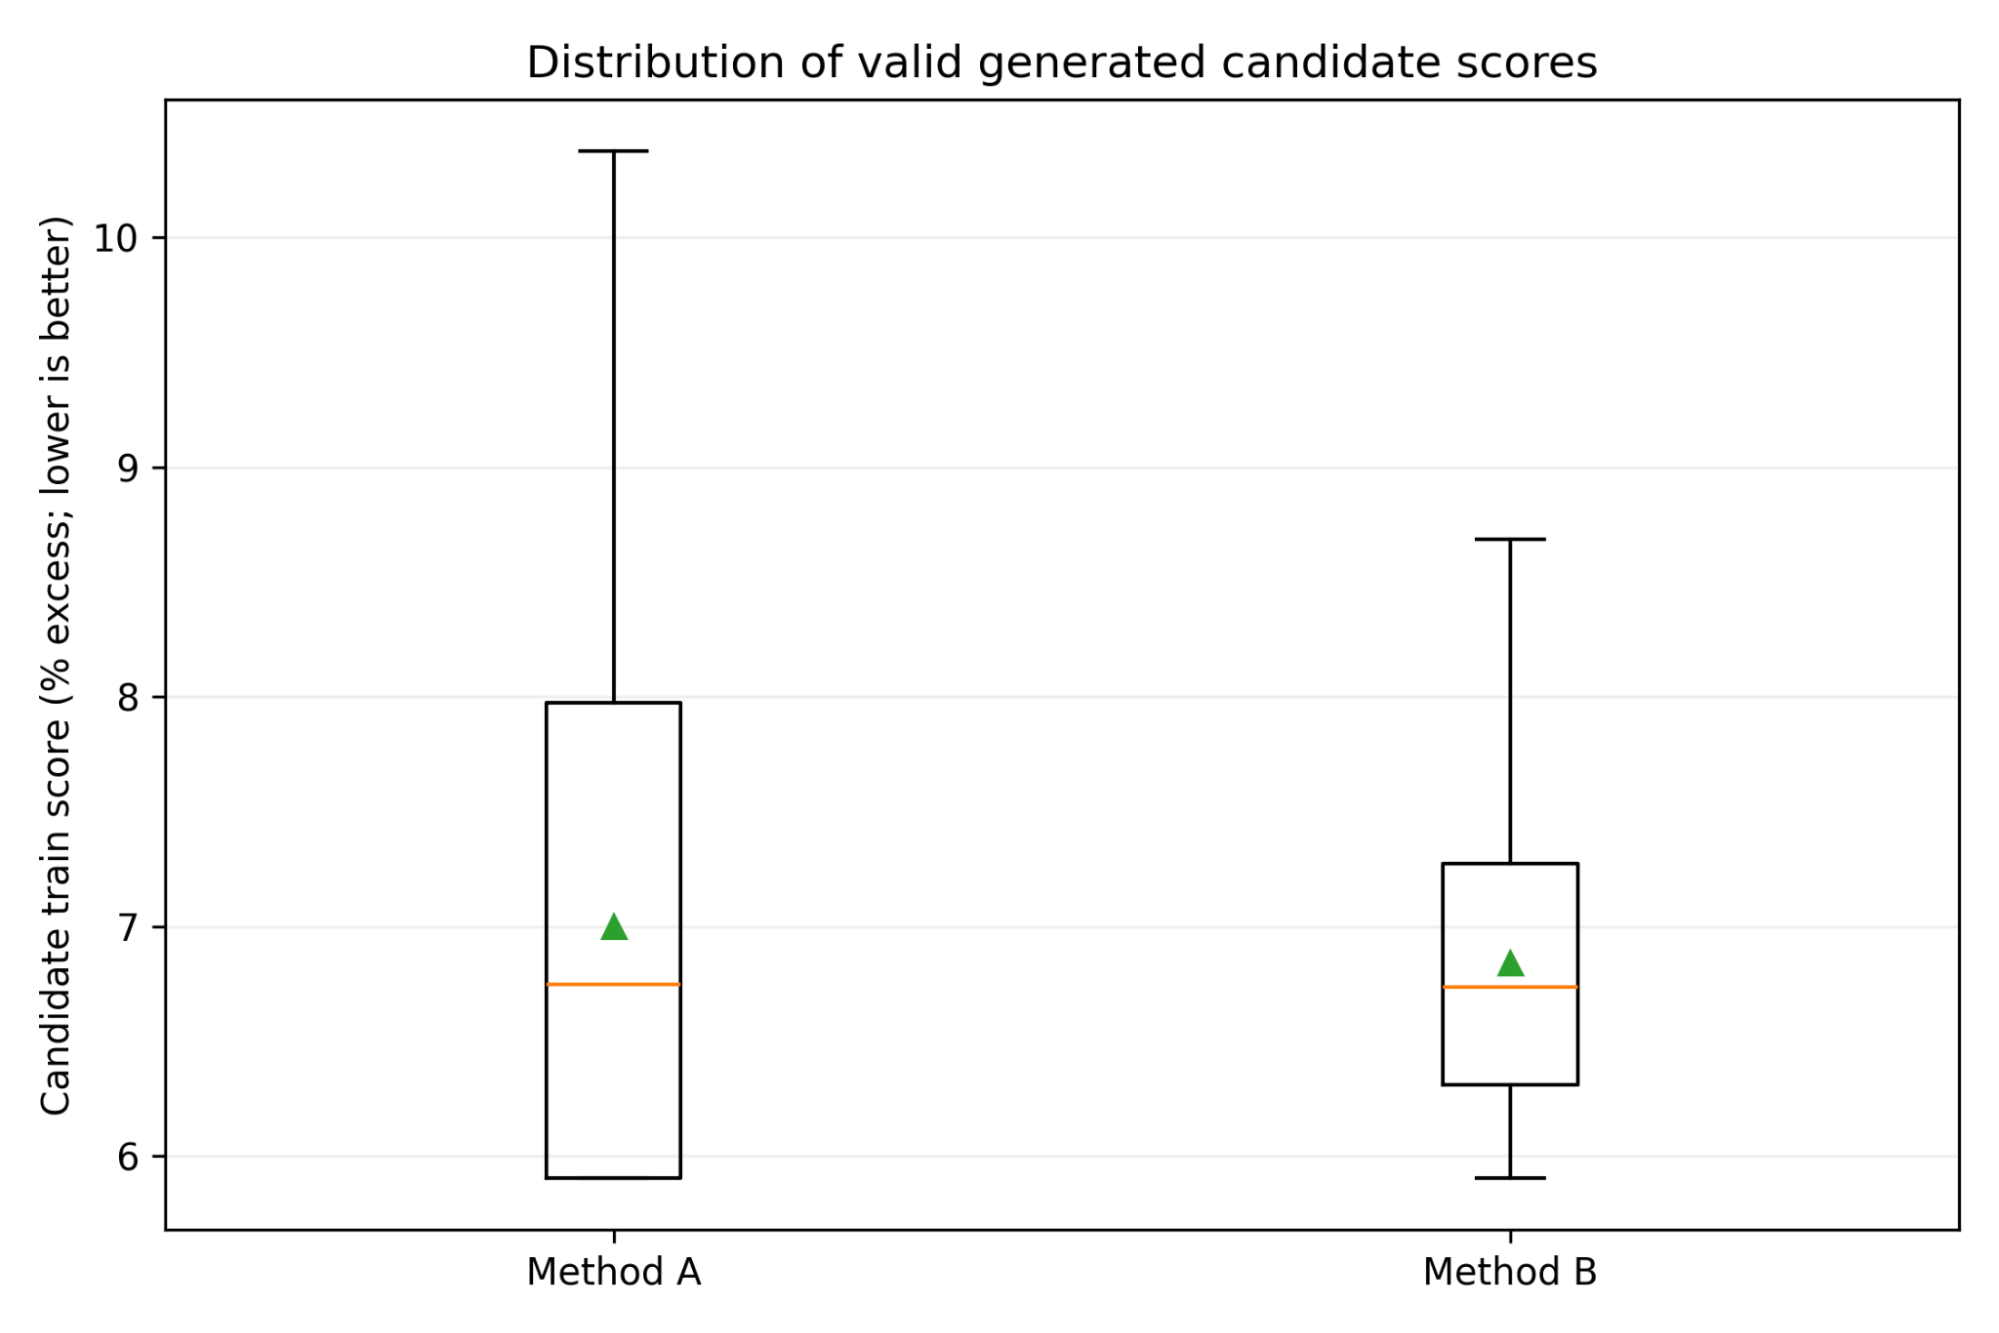
\includegraphics[width=\linewidth]{images/Figure 3(b).png}
        \small (b) Distribution of valid candidate scores
    \end{minipage}
    \caption{Main experiment: (a) best-so-far training score against cumulative tokens used and (b) distribution of valid generated candidate scores.}
    \label{fig:main}
\end{figure}


\section{Discussion}
\subsection{Effectiveness of Evolutionary Feedback}
The first research question investigated whether evolutionary feedback could discover better bin-packing heuristics than independent sampling under a fixed LLM token budget.
Firstly, as shown in Table~\ref{tab:runs} and Figure~\ref{fig:main}(b), Method B achieved lower mean training scores and a narrower interquartile range than Method A, suggesting better and more consistent candidate generation. This may be because incorporating promising candidates into subsequent prompts directs the LLM away from poor programs and allows it to build upon previously successful solutions. Secondly, Method A achieved marginally better best training scores in both repetitions, although the differences were negligible. Figure~\ref{fig:main}(a) shows that neither method achieved substantial improvements as token consumption increased. Furthermore, Method B generated fewer valid candidates due to the additional prompt tokens required for parent programs. Ultimately, both methods selected Best Fit in all four runs. This demonstrates that better average candidate quality does not necessarily translate into discovering a better final heuristic. Under the tested token budget, evolutionary feedback offered no meaningful advantage over independent sampling in final solution quality.
\subsection{Generalisation to Unseen Distributions}
The second research question investigated whether evolutionary feedback affects generalisation to unseen item-size distributions, instance sizes and item orderings. As both methods achieved identical ID and OOD test performance because all four runs selected Best Fit, no observable generalisation difference between the methods was found. Despite this, OOD evaluation results showed that heuristic performance varied across instance families, underlining the influence of item characteristics and ordering on bin-selection strategies.

Furthermore, training and validation contained the same distribution families, although different random seeds prevented instance-level overlap. Consequently, validation-based selection may favour candidates suited to familiar distributions rather than unseen ones. Further evaluation of newly discovered heuristics would be necessary to establish whether either method produces more generalisable solutions.

\subsection{Comparison with Established Baselines}
The comparison against First Fit, Best Fit and tuned ab-First Fit highlights the difficulty of discovering improved bin-packing heuristics. Although Best Fit provided a competitive starting point, no single baseline performed best across all instance families, with performance varying according to item-size distributions and ordering. Again, neither search method improved upon Best Fit despite the allocated token budget. This suggests that with our current set up, discovering priority functions that consistently outperform established heuristics across diverse instances remains challenging. Future work could explore more diverse training distributions and alternative search strategies to encourage the discovery of more generalisable heuristics.
\section{Limitations and Future Work}
 One limitation was that a fixed token budget of about 500,000 tokens per run was used  to control LLM usage and costs. This restricted the number of candidates generated, particularly for Method B, which required additional prompt tokens to include parent programs. Consequently, Method B generated fewer candidates than Method A despite achieving better average candidate performance. Future work could compare the methods across different token budgets to investigate how additional search expenditure affects candidate quality and whether either method benefits more from a larger budget.
Another limitation was the limited exploration of different LLM models and search configurations, where the experiments used a single LLM and fixed generation settings. Although different parent-selection temperatures were explored during the pilot study, the final experiments used a selection temperature of 1.0 for Method B. Therefore, the findings may not generalise to other models or configurations. Future work could evaluate different LLMs, generation temperatures and parent-selection strategies to determine whether alternative configurations improve heuristic discovery.
\section{Conclusion}
This study compared independent sampling (Method A) and LLM-guided evolutionary feedback (Method B) for discovering online bin-packing heuristics under a fixed token budget. Although Method B generated candidates with better average training performance and lower variability, Method A achieved marginally better training scores and produced more valid candidates. However, neither method outperformed Best Fit, with all four runs selecting Best Fit and achieving identical performance across in-distribution and out-of-distribution test instances. These findings suggest that evolutionary feedback may improve average candidate quality but does not necessarily lead to better final heuristics or generalisation under a fixed token budget.

% ===== REFERENCES =====
\begin{thebibliography}{99}

\bibitem{romera2023}
Romera-Paredes, B., Barekatain, M., Novikov, A., Balog, M.,
Kumar, M. P., Dupont, E., Ruiz, F. J., Ellenberg, J. S.,
Wang, P., Fawzi, O., Kohli, P., \& Fawzi, A. (2023).
Mathematical discoveries from program search with large language models.
\textit{Nature}, \textit{625}(7995), 468--475.
\url{https://doi.org/10.1038/s41586-023-06924-6}

\bibitem{chen2026}
Chen, H., Qi, X., Zhao, J. X., Feng, Z., Liu, S.,
Xu, K., Koh, P. W., \& Hooi, B. (2026).
\textit{Frugalevo: Towards Cost-Aware LLM-Guided Program Evolution}.
\url{https://doi.org/10.48550/arXiv.2610.03675}

\bibitem{huang2025}
Huang, Z., Wu, W., Wu, K., Lee, W.-B., \& Wang, J. (2025, May 18).
\textit{CALM: Co-Evolution of Algorithms and Language Model
for Automatic Heuristic Design}.
\url{https://doi.org/10.48550/arXiv.2505.12285}

\bibitem{sim2025}
Sim, K., Renau, Q., \& Hart, E. (2025, April 17).
Beyond the hype: Benchmarking LLM-evolved heuristics for Bin Packing.
\textit{Lecture Notes in Computer Science}, 386--402.
\url{https://doi.org/10.1007/978-3-031-90065-5_24}

\bibitem{herrmann2026}
Herrmann, J., \& Pallez, G. (2026).
An in-depth study of LLM contributions to the Bin Packing Problem.
\textit{ACM Transactions on Evolutionary Learning and Optimization}.
\url{https://doi.org/10.1145/3821574}

\end{thebibliography}

\end{document}
